\addchapheadtotoc
\chapter{Background on Radiation in Combustion}\label{chapter:Importance}

\section{Fundamentals of radiation} \label{Sec:FundOfRad}
Thermal radiation is the transfer of thermal energy through through electromagnetic waves, according to electromagnetic wave theory, and by particulate photons, according to quantum mechanics. 
Either perspective may be more convenient for a given circumstance, but both perspectives are required for a complete definition \cite{Modest2013RadiativeTransfer}. The transfer of energy occurs at the speed of light, which is $2.998 \times 10^8$ meters per second in a vacuum.
Much faster than most processes, and often believed to be a theoretical speed limit of the universe.

The effects of thermal radiation can be seen in every day life. Common examples include the sun, a campfire, and a hot pavement. 
Wavelengths are usually from picometers ($10^{-12}$ m) for gamma rays to megameters ($10^6$ m) for ultra-low frequency radio waves.
For combustion systems, where temperatures typically fall between 2000 and 2500K, relevant wavelengths generally fall between 1 and 15 $\mu{}$m ($10^{-6}$ m), in the infrared and visible light parts of the spectrum \cite{Liu2020TheFlames}.

Thermal radiation is known to have an \textit{all-to-all} nature. Radiation emitted at one point has the ability to reach another point very far away. 
This is in contrast to conductive and convective modes of heat transfer where thermal energy is transferred through direct contact and fluid motion (local phenomena). 
It is for this reason that radiation plays a very important role in massive-scale studies such as in the vacuum of space.
A brief description of various fundamental laws are presented,
readers should review referenced texts for more thorough descriptions \cite{Howell2010ThermalTransfer,Modest2013RadiativeTransfer}.

\subsection{Basic Laws of radiation}

\subsubsection{The idealized 'Black body'}
A body which absorbs perfectly cannot be seen and must therefore be black. Therefore, the term \textit{black body} refers to the an ideal absorber, upon which any incident light of any wavelength will be absorbed in its entirety. In addition, according to arguments posed in \ref{sec:KirchoffsLaw}, black-bodies are also ideal emitters.
The ideal nature of black bodies provides a useful basis for radiation calculations, and therefore appears often in radiation-relevant literature.

Assuming matter can only exist at discrete energy states, Max Planck derived the black body emissive power spectrum (Planck's law), shown in eq. \ref{eq:PlancksLaw}.
\begin{equation}
    E_{bv}(T,\nu{}) = \frac{2\pi{}h\nu{}^3n^2}{c_0^2\left[e^\frac{h\nu{}}{kT}-1\right]}
    \label{eq:PlancksLaw}
\end{equation}
Where $h$ is Planck's constant, $\nu{}$ is the wave frequency, $n$ is the refractive index of the medium, $c_0$ is the speed of light in a vacuum, $k$ is the Boltzmann constant, and $T$ is temperature. This equation can be integrated across the electromagnetic spectrum to produce an approximation for the net emissive power from a black body, as shown in eq. \ref{eq:PlancksLawIntegrated}.
\begin{equation}
    E_b(T) = n^2\sigma{}T^4
    \label{eq:PlancksLawIntegrated}
\end{equation}

While emissive power is an important quantity for radiation modeling, the radiative intensity, $I$, or emissive power per unit solid angle is a more convenient quantity for many radiation problems. A "solid angle" is a description of a differential area along the unit sphere, similar to a two-dimensional angle on the unit circle. The definition for intensity from a diffuse emitter is eq. \ref{eq:Intensity}.
\begin{equation}
    I_b(T) = \frac{E_b(T)}{\pi}
    \label{eq:Intensity}
\end{equation}


\subsubsection{Kirchhoff's Law} \label{sec:KirchoffsLaw}
Two systems are constructed consisting of an enclosure of black surfaces surrounding an object. The object in the first system is a black-body, and the object in the second system is a gray body (emits a fraction of the energy a black body emits). Both systems are thermally insulated to the surroundings. 
According to the second law of thermodynamics, the temperatures in both systems will equalize to a constant value. This implies that the energy emitted and absorbed by each object should be the same.
Since a black body is a better absorber than the gray body, it must also be a better emitter. This argument can be proposed for any variation of the gray body. Therefore, the black-body must also be the best possible emitter of radiation.
Further continuation of this argument reveals that the ratio of emission of any object to that of a black body, the emissivity, must also equal the ratio of the absorption of that object to that of a black body, the absorptivity. This argument applies for emission at any wavelength and any direction for ingoing or outgoing electromagnetic rays, therefore establishing the equality of spectral, directional emissivity $\epsilon_{\eta{}\theta{}}$ and spectral, directional absorptivity $\alpha{}_{\eta,\theta}$ at thermal equilibrium, as shown in eq. \ref{eq:KirchhoffsLaw}.
\begin{equation}
    \epsilon{}_{\eta{},\theta{}}=\alpha{}_{\eta{},\theta{}}
    \label{eq:KirchhoffsLaw}
\end{equation}


\subsection{Thermal radiation in participating media} \label{section:RTE}
For combustion systems, thermal radiation interacts with the media as well as the walls. The fundamental equation to describe radiation in an absorbing-emitting medium is the radiative transfer equation (RTE), eq. \ref{eq:RTE2}.

\begin{equation}
    \frac{dI_\eta{}}{d\hat{\textbf{s}}} = \hat{\textbf{s}} \cdot \nabla{I_\eta{}} = \kappa{}_\eta{}I_{b\eta{}}-\kappa{}_\eta{}I_\eta{}-\sigma{}_{s\eta{}}I_\eta{}+\frac{\sigma{}_{s\eta{}}}{4\pi}\int_{4\pi{}}{I_\eta{}(\hat{\textbf{s}})\Phi_\eta{}(\hat{\textbf{s}}_i,\hat{\textbf{s}})}\,d\Omega{}_i
    \label{eq:RTE2}
\end{equation}

Where $I$ is ray intensity, $\hat{\textbf{s}}$ is a path length (with both a direction and a location), $\kappa{}$ is the absorption coefficient, $I_b$ is the black-body intensity, $\sigma{}$ is the scattering coefficient, and $\Phi{}$ is the scattering phase-function (representing the probability a ray from direction $\hat{\textbf{s}}_i$ is scattered into direction $\hat{\textbf{s}})$. Subscript $\eta{}$ represents wavenumber (the inverse of wavelength) and $i$ marks an incident direction. 
This equation describes how the intensity of a pencil of rays changes along a path length $\hat{\textbf{s}}$. A ray intensity will decrease due to absorption ($\kappa{}_\eta{}I_\eta{}$, also known as Beer's law) and out-scattering ($\sigma{}_{s\eta{}}I_\eta{}$). And the ray intensity will increase due to further emission along the path-length ($\kappa{}_\eta{}I_{b\eta{}}$) and scattering of rays from other directions into the path length of interest ($\frac{\sigma{}_s}{4\pi}\int_{4\pi{}}{I_\eta{}(\hat{\textbf{s}})\Phi_\eta{}(\hat{\textbf{s}}_i,\hat{\textbf{s}})}\,d\Omega{}_i$). 

The existence of both an integral and a differential in eq. \ref{eq:RTE2} contributes to the complexity of the problem as the equation being modeled is an integro-differential equation. 
This requires both modeling of local phenomena and the influence of global phenomena on local conditions. 
This all-to-all nature is the reason for the immense computational difficulty of modeling the RTE. 
In addition, as will be explained in section \ref{Sec:Nongray}, the highly intermittent nature of the emission spectrum of gas imposes an additional modeling difficulty.

Absorption coefficient, $\kappa_{\eta{}}$ and scattering coefficient $\sigma{}_\eta{}$ are often combined into the extinction coefficient $\beta{}_\eta{}$. Equation \ref{eq:RTE2} can then be rewritten to \ref{eq:RTErewritten}.
\begin{equation}
    \frac{dI_\eta{}}{d\hat{\textbf{s}}} = \beta{}_\eta{}[S(\hat{\textbf{s}}',\hat{\textbf{s}})-I_\eta{}]
    \label{eq:RTErewritten}
\end{equation}
\begin{equation}
    S(\hat{\textbf{s}}',\hat{\textbf{s}}) = (1-\omega{}_\eta{})I_{b\eta{}}+\frac{\omega{}_\eta{}}{4\pi}\int_{4\pi{}}{I_\eta{}(\hat{\textbf{s}})\Phi_\eta{}(\hat{\textbf{s}}_i,\hat{\textbf{s}})}\,d\Omega{}_i
    \label{eq:RTE_S}
\end{equation}
Where $S_\eta{}(\hat{\textbf{s}}',\hat{\textbf{s}})$ is the ray-intensity source term eq. \ref{eq:RTE_S}, and $\omega{}_\eta{}=\sigma{}_{s\eta{}}/\beta_{\eta{}}$ is the single-scattering albedo. Eq. \ref{eq:RTErewritten} shows that the intensity of the pencil of rays increases due to a source term, and decreases proportional to it's current intensity.
The extinction coefficient $\beta{}$, is often divided from both sides of eq. \ref{eq:RTE2}, and the resulting $\beta{}d\hat{\textbf{s}}$ term is called the optical distance, $d\tau{}_\eta{}$.

The RTE can be integrated along an optical path length resulting in eq. \ref{eq:RTE_Solution}.
\begin{equation}
    I_\eta{}(\tau{}_\eta{}) = I_\eta{}(0)e^{-\tau{}_\eta{}}+\int_{0}^{\tau{}_\eta{}}{S_\eta{}(\tau{}'_\eta{},\hat{s})e^{-(\tau{}_\eta{}-\tau{}'_\eta{})}}d\tau{}'_\eta{}
    \label{eq:RTE_Solution}
\end{equation}
Equations \ref{eq:RTE2} and \ref{eq:RTE_Solution} display an important trait in thermal radiation that is conceptually obvious, but has significant consequences on the modeling procedure:
the change in intensity is a function of the current intensity. In other words, the intensity of a pencil of rays at one location cannot be known without knowledge of the ray's intensity directly before.
As a result, one cannot accurately predict the variation of intensity in space without tracing a ray sequentially through every point between where it is emitted, and the point of interest.
This ordered nature is forces the raytracing procedure to occur iteratively through the mesh.

A very simple example of radiative heat transfer can be applied to a non-scattering, isothermal sphere that is surrounded by cold, black walls. 
The emanating intensity can be described by eq. \ref{eq:emitting_sphere}.
\begin{equation}
    I_\eta{}(\tau{}_R,\theta{}) = I_{b\eta{}}\left(1-e^{-2\tau{}_R\cos{\theta}}\right)
    \label{eq:emitting_sphere}
\end{equation}
Where $\tau{}_R$ is the optical radius of the sphere and $\theta{}$ is the exit angle (angle between the exit direction and the norm of the internal face of the sphere).
Then, the radiative heat flux can be evaluated by integration over all exit angles, azimuthal angles, and wavenumbers.
\begin{equation}
    \textbf{q}=\int_0^\infty{}\int_0^{2\pi}\int_0^{\pi{}}I_\eta{}(\tau{}_R,\theta)\cos{\theta}\sin{\theta}~d\theta{}~d\psi{}~d\eta{}
    \label{eq:heatflux}
\end{equation}
\begin{equation}
    \textbf{q}=\int_0^\infty{}\int_0^{2\pi}\int_0^{\pi{}}I_{b\eta{}}\left(1-e^{-2\tau{}_R\cos{\theta}}\right)\cos{\theta}\sin{\theta}~d\theta{}~d\psi{}~d\eta{}
    \label{eq:heatflux}
\end{equation}
\begin{equation}
    \textbf{q}=n^2\sigma{}T^4\left\{1-\frac{1}{2\tau{}_R^2}\left[1-(1+2\tau{}_R)e^{-2\tau{}_R}\right]\right\}
    \label{eq:heatflux}
\end{equation}
Under the conditions of an optically thin sphere, radiative re-absorption can be ignored, and the equation can be simplified to
\begin{equation}
    \textbf{q}=n^2\sigma{}T^4\frac{4}{3}\tau{}_R.
    \label{eq:heatflux}
\end{equation}
Where the heat flux can be integrated across the surface area of the sphere to produce the net energy emitted.
\begin{equation}
    Q_{emi}=4\kappa{}n^2\sigma{}T^4V
    \label{eq:RadEmis}
\end{equation}
This equation can be generalized to define the emission from any isothermal volume, and is often used to define the net energy emitted from a computational cell using the Monte-Carlo Ray Tracing method.

\subsection{Spectral effects}\label{Sec:Nongray}
Like all substances, gases emit radiation along the electromagnetic spectrum. Under most conditions for combustion phenomena, radiative emission is isolated to the infrared part of the spectrum, between wavelengths of 1 to 15 $\mu{}$m \cite{Liu2020TheFlames}.

The black body spectrum in section \ref{Sec:FundOfRad} can approximate the emission spectrum of many solid materials, but is inadvisable to be used for gas emission. 
Most solid structures have a multitude of modes of oscillations, from the crystal-lattice structure down to the molecular energy states \cite{Viskanta1975HeatSolids}. As a result, the emission spectrum of solids is often continuous and can be approximated as a constant fraction of the black body emission spectrum (gray) \cite{Howell2010ThermalTransfer}. 
Gases, however, are restricted to the oscillation modes from the natural energy states of the molecules in the mixture. Quantum mechanics postulates that these energy states are discrete, and therefore the change in energy states and resulting emission frequencies must also be discrete \cite{Hanson2016SpectroscopyGases}.
\begin{figure}
\centering
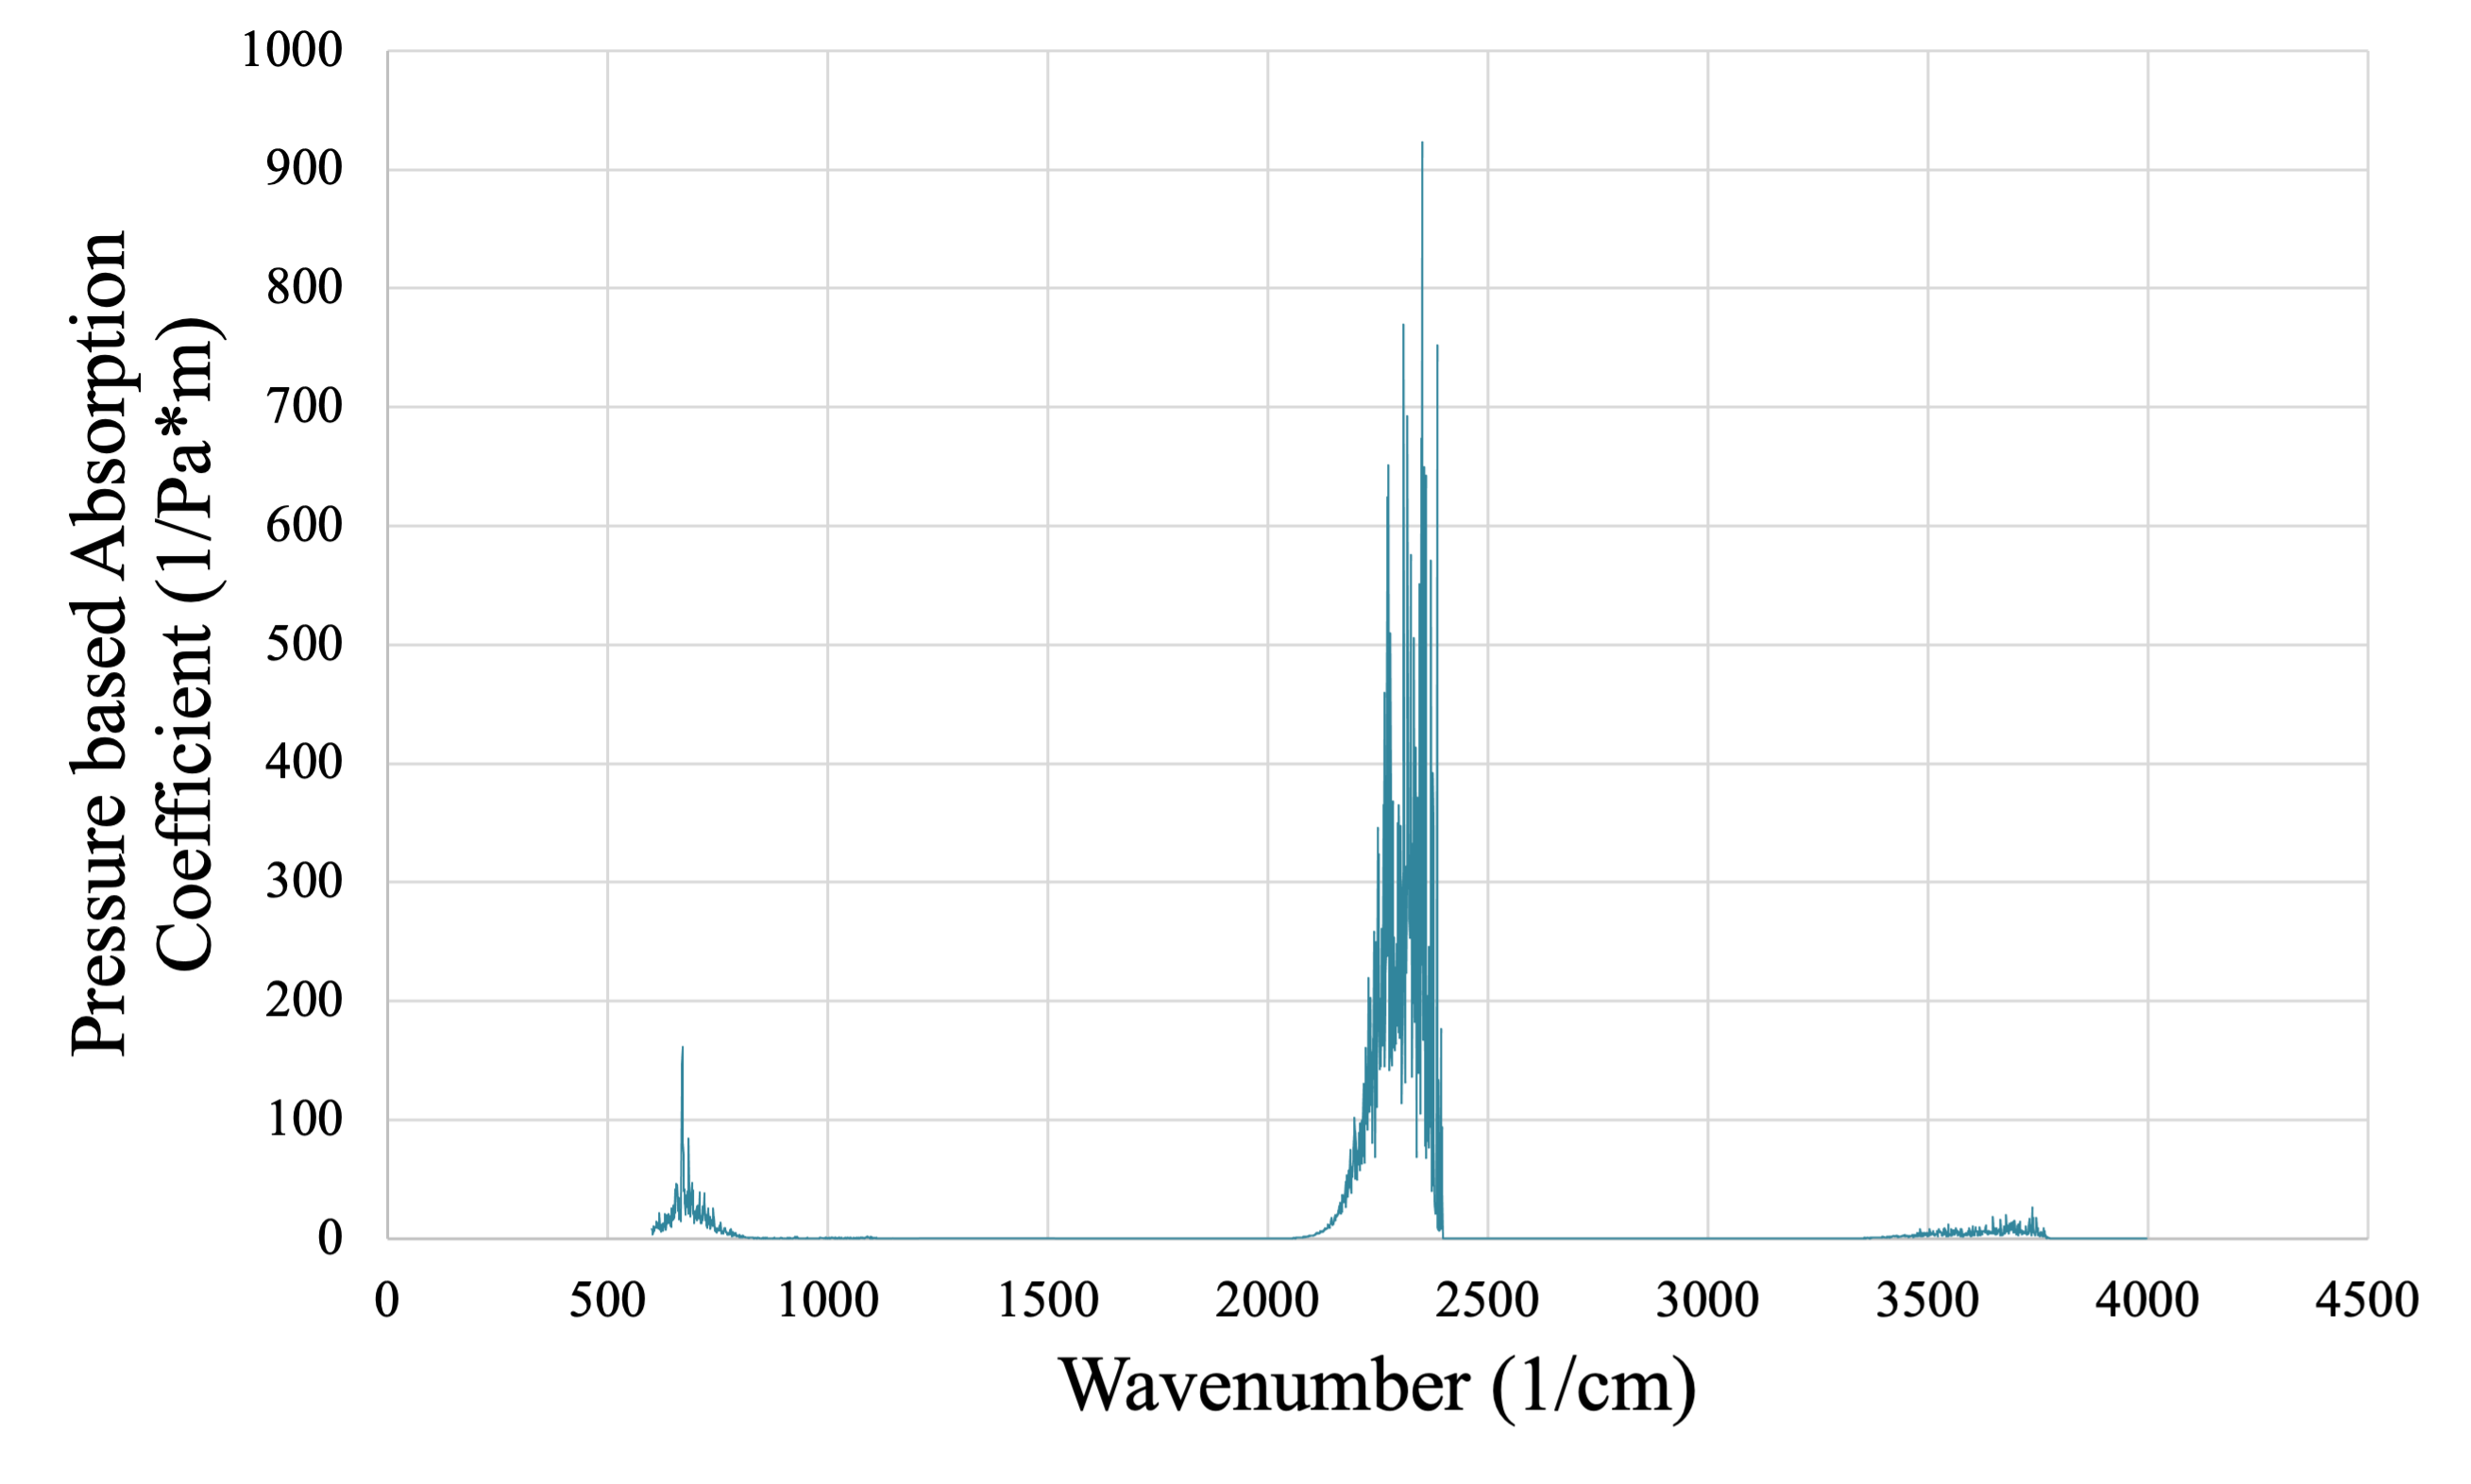
\includegraphics[width=0.8\linewidth]{figures/ch2/SpectralLinesCO2.png}
\caption{Spectrals lines of CO$_2$ at $1$ bar and $1600$ K }
\label{fig:SpectralLines}
\end{figure}


The largest molecular contributors to emission in most hydrocarbon flames are $CO_2$, $CO$, $H_2O$, and soot. Figure \ref{fig:SpectralLines} shows the absorption coefficient spectrum of CO$_2$. 
\textit{Ab initio} modeling and empirical evidence can be used to obtain approximations for the emission spectra of a molecule at a specified pressure and temperature. This information has been collected into a series of available online databases \cite{Rothman2010HITEMPDatabase}. 
Those databases can then be used to provide a radiation solver absorption coefficients as a function of chemical mixture composition and thermodynamic state.

While the emission spectrum of gases is discrete, the radiation from many flames have been observed to be much more continuous \cite{Modest2013RadiativeTransfer}. This is a direct result of the emission of soot.
Soot particles are generated through the agglomeration of unburnt hydrocarbons. The resulting particulates contribute much to the visual glow seen in flames. 
Soot particles have sizes of only tens of $\mu{}$m, and volume fractions of only $10^{-4}$\% to $10^{-6}$\%, but often contribute the majority of radiation from a flame \cite{Modest2013RadiativeTransfer}.

\subsection{Characterizing the contribution of radiation}
Understanding relative influence of radiation compared against other forms of energy transfer is a necessary task for many scientists and engineers, however a complete solution to the RTE alongside within their simulated domain (eq. \ref{eq:RTE2}) is often unnecessary to accomplish this. 
There exist several parameters and non-dimensional relationships which can adequately characterize its magnitude in relation to other relevant parameters.

One approach would be to determine the tendency for a medium to absorb any emitted radiation. The diminishment of intensity of a pencil of rays due to absorption can be evaluated as in eq. \ref{eq:DiminishmentOfRayIntensity}.
\begin{equation}
    I_\eta{}(s)=I_\eta{}(0)\exp{\left(-\int^\infty_0{\kappa{}_\eta{}~ds}\right)}
    \label{eq:DiminishmentOfRayIntensity}
\end{equation}
The quantity in the exponential is known as the optical thickness, $\tau{}_\eta{}$ which is essentially a description of the opacity of a medium. It is a function of not only the tendency for a fluid element to absorb the energy of passing radiation, defined by the absorption coefficient, but also the overall distance over which the ray can be absorbed.
If one assumes the absorption coefficient remains constant along the path length, $s$, the equation for optical thickness can be reduced to eq. \ref{eq:Tau_simple}.
\begin{equation}
    \tau{}_\eta = \kappa{}_\eta{}\Delta{s}
    \label{eq:Tau_simple}
\end{equation}
The dimension of absorption coefficient is $m^{-1}$. Therefore, the optical thickness is a non-dimensional parameter that defines the propensity for a medium to absorb any emitted radiation, and can be a useful term to predict the necessity of solving the RTE. 
Optical thickness values of $2.303$, $4.605$, and $6.908$ define the optical distances necessary to diminish intensities by $90$\%, $99$\%, and $99.9$\%, respectively.
Media which tend to absorb very little are known as \textit{optically thin}, and can be modeled using the \textit{optically thin assumption (OTA)}, where radiation contributes a simple volumetric energy loss to the local fluid differential volume, and any radiative absorption is ignored.
Media with high absorption coefficients and/or long length scales are known as \textit{optically thick}. Under these circumstances the absorption component of the RTE becomes more significant and must be modeled.
Very optically thick media that find radiative re-absorption to occur on very small length scales relative to the geometry can model radiation using the \textit{diffusion approximation}, where radiative heat transfer is assumed to act similar to conductive diffusion with a radiative conductivity coefficient acting in place of the coefficient of thermal conductivity. 
Under moderate absorption coefficients, the full RTE must be modeled for both emission and absorption throughout the volume \cite{Modest2013RadiativeTransfer}.

Many instances of radiative gases call for an averaged quantity of absorption coefficient across the spectrum. The Planck-mean absorption coefficient, eq. \ref{eq:PlanckMean}, is often used in this context.
\begin{equation}
    \kappa{}_p = \frac{\int^\infty_0{\kappa{}_\eta{}I_{b,\eta}~d\eta}}{\int^\infty_0{I_{b,\eta}~d\eta}}=\frac{\pi}{\sigma{}T^4}\int^\infty_0{\kappa{}_\eta{}I_{b,\eta}~d\eta}
    \label{eq:PlanckMean}
\end{equation}
Separate Planck-mean absorption coefficients can be defined for each of the more significant radiatively participating components of the mixture (often CO$_2$, H$_2$O, CO, CH$_4$, and soot). The net Planck-mean absorption coefficient can then be evaluated as a summation of each, weighted by their respective mole fractions.
A simplified optical thickness, finally, can be defined as $\tau{}=\kappa{}_p\Delta{s}$.

The comparison of radiative and chemical heat generation terms can also provide perspective as to its relevance. As discussed by \citet{Liu2020TheFlames}, the radiant fraction can be used for this, eq. \ref{eq:RadiantFraction}.
\begin{equation}
    \chi{}_R=\frac{\dot{Q}_{emi}-\dot{Q}_{abs}}{\dot{Q}_{chem}}=\frac{\int_V{4\pi{}\kappa{}_p\sigma{}T^4~dV}-\int_V\left[\int_0^\infty{\left(\kappa{}_\eta{}\int_{4\pi}I_\eta{}~d\Omega\right)~d\eta{}}\right]~dV}{\rho{}_Fu_F\Delta{h}_c\pi{}d_F^2/4}
    \label{eq:RadiantFraction}
\end{equation}
Where the numerator defines the radiative divergence of heat flux, and the denominator quantifies the contribution of heat through chemistry within the flame. $d_F$ and $u_F$ are a length scale and representative velocity for the system.
The definition can be reformulated into eq. \ref{eq:RadiantFraction_reformulated}.
\begin{equation}
    \chi{}_R=\left(\frac{4V_fl}{\pi{}u_Fd_F^2}\right)\left(\frac{4\kappa{}\sigma{}T_p^4}{\rho{}_F\Delta{h}_c}\right)\left(1-\frac{\dot{Q}_{abs}}{\dot{Q}_{emi}}\right)
    \label{eq:RadiantFraction_reformulated}
\end{equation}
In this format, the three terms included can be separately considered. The first term considers the flow residence time. Larger volumes and slower velocities result in a longer period for radiation to have its effect.
The second term is inverse of the characteristic radiation cooling time. 
The third term is the flame transparency. This term quantifies degree of re-absorption in the fame. A high degree of re-absorption will have a lower flame transparency. 

It should be noted that additional parameters may be used to estimate the importance of other effects, such as radiative pressure and radiative energy density.
While the contribution of these effects are generally small under most conditions studied in combustion, they should be considered under extreme circumstances, and the reader should consult representative texts for further information in this context \cite{Pai1966RadiationDynamics}.

\subsection{Frozen-Field Analysis}
A \textit{frozen-field analysis} is one approach used in many thermal radiation models. In frozen-field analysis, it is assumed that the time required for a given ray to propagate across the domain is extremely small relative to even the shortest computational time-steps. 
As a result, the temporal evolution of parameters in the system can be assumed negligible during a ray's travel.
This greatly simplifies the solution to the radiative transfer equation (eq. \ref{eq:RTE2}, which is already presented with temporal-evolution neglected), as it can now be modeled at any given time-step of the CFD solution, while assuming the radiation solution can be calculated using a single timestep.

\section{Effect of radiation in combustion systems}
Radiation presents a variety of influences in combustion systems from both a physical and modeling perspective. A variety of these influences will be discussed in this section. First, the direct influences on fluid-dynamics are presented, followed by influences specific to turbulent flows, within the enclosing walls or surrounding objects, and to the chemical propagation and product mixture compositions.

\subsection{On fluid motion – TODO}
Many fluid dynamical systems see a relevant contribution of radiation. These physics that are present with non-chemically reacting flows can present themselves equally or in greater magnitude in reacting flows, and therefore provide a useful initial basis to define the influence of radiation in combustion. 

In general, any systems with high temperature fluid dynamics can see a powerful influence of radiation, and its resulting effects. 
Radiation is more pronounced in systems which have high residence times, where the relatively slow timescales of radiative heating have more time to influence the system \cite{Wu2021LimitationsFires}. 
To a degree, any gas-dynamical system with high temperatures and relatively low densities will exhibit high degrees of radiative emission compared to conduction and convection \cite{Pai1966RadiationDynamics}. This includes the fields of hypersonics, fission and fusion nuclear energy, and space exploration.

For non-chemically reacting systems, the gasdynamical influences of radiation take effect often in regimes of science well-beyond those seen in every day life. Under atmospheric conditions, for example, the influence of radiation is largely negligible compared to that of conduction and convection \cite{Pai1966RadiationDynamics}.
Even under hypersonic conditions, such as inter-continental ballistic missiles (ICBMS), radiation is often still an order of magnitude lower than aerodynamic heating. Only at temperatures seen by re-entry vehicles (10$^4$ K) does radiation have a strong, non-negligible effect.
In nuclear systems, such as nuclear fusion reactors, where temperatures reach 10$^6$K, the influence of the radiation becomes extremely significant. This follows from not only its redistribution of energy, but also its influence on pressure (through momentum imparted via photon collisions) and the radiative energy density become non-negligible as well. 



Combustion sees a redistribution of thermal energy as a result of radiation. 
Neglecting thermal radiation may lead to large over-predictions of flow temperature by upwards of 200K in some cases \cite{Modest2016RadiativeSystems,Wu2021LimitationsFires,Coelho2018RadiativeSystems}, as well as under-predictions of flame temperature in others. The resulting influence on the thermodynamics and fluid dynamics of the system may be considerable.

Buoyancy effects
Microgravity effects
Dr. Zhaos paper



\subsection{On turbulence}
The modeling of disparate time and length scales involved with turbulent fluctuations in many fluid dynamic systems presents a problem for many computational scientists.
Resolving all of these scales would require extremely well resolved grid, often to an infeasible degree computationally. 
Instead, a coarser grid is often used, with properties defined by an average over that of the contained fluid structures. This is the approach used in Reynold's Averaged Navier Stokes (RANS) modeling and Large Eddy Simulations (LES).
The averaging of the governing equations of fluid dynamics, however, presents another difficulty, as many non-linear terms cannot be well represented by a linear average over thermodynamic parameters.
This problem emerges in turbulent modeling of radiation, and is often called Turbulence-Radiation Interaction (TRI).

The transport of radiation can be divided into processes of emission and absorption. 
Within a semi-transparent medium, or any surface-surface exchange of radiation, the emission and absorption are defined by a non-linear functions of the thermodynamic conditions in the medium.
Equation \ref{eq:DivHeatFlux} is the divergence of heat flux due to radiation. It defines the contribution of radiation to a differential volume, and its negative represents the volumetric energetic source term in the energy equation for fluid dynamics.
\begin{equation}
    -S_{rad}=\nabla\cdot{}q_{rad} = \int_0^\infty{\left(4\pi{}\kappa_\eta{}I_{b\eta{}}-\int_{4\pi}{\kappa{}_\eta{}I_\eta{}~d\Omega{}}\right)~d\eta{}}
    \label{eq:DivHeatFlux}
\end{equation}
The averaging process will reformulate the equation into the following, eq. \ref{eq:AvgDivHeatFlux}.
\begin{equation}
    -S_{rad}=\langle\nabla\cdot{}q_{rad}\rangle = \int_0^\infty{\left(4\pi{}\langle\kappa_\eta{}I_{b\eta{}}\rangle-\int_{4\pi}{\langle\kappa{}_\eta{}I_\eta{}\rangle~d\Omega{}}\right)~d\eta{}}
    \label{eq:AvgDivHeatFlux}
\end{equation}
The simple change introduces a significant complexity into the system. The distinction can be described in eq. \ref{eq:AbsTRI} and \ref{eq:EmiTRI}.
\begin{equation}
    \text{Absorption TRI:~~}\langle\kappa_\eta{}I_{\eta}\rangle \neq \kappa_\eta{}(\langle\phi{}\rangle) I_{\eta}(\langle{}T\rangle{})
    \label{eq:AbsTRI}
\end{equation}
\begin{equation}
    \text{Emission TRI:~~}\langle\kappa_\eta{}I_{b\eta}\rangle \neq \kappa_\eta{}(\langle\phi{}\rangle) I_{b\eta}(\langle{}T\rangle{})
    \label{eq:EmiTRI}
\end{equation}
Where $\phi{}$ is a vector defining the chemical composition of the mixture. Therefore, absorption and emission TRI refers to the modeling technique used to estimate the left-hand side terms in eqs. \ref{eq:AbsTRI} and \ref{eq:EmiTRI}.

As a simple demonstration, the total intensity emitted from a black-body is defined by eq. \ref{eq:PlancksLawIntegrated} and \ref{eq:Intensity}.
An apparent relationship between the emission and $T^4$ captures the first problem, as $\langle{T}\rangle^4 \neq \langle{}T^4\rangle$. 
The consequences of which may be conceptualized easily. Many turbulent combustion systems exhibit a high degree of fluctuations in temperature. Even within the length-scale of a computational cell, a flame-thickness may be small enough that there may exist a pocket of product mixture alongside an cooler, unburnt gas.
Therefore, one can expect a higher degree of emission than predicted after an evaluation of $\langle{T}\rangle^4$, an phenomenon which becomes apparent when comparing radiation from a fully resolved Direct Numerical Simulation (DNS) and averaged simulations (RANS, LES) with no TRI.
Similar arguments can be made regarding the influence of the absorption coefficient on emission, as it is also a nonlinear function of chemical composition and temperature.

The influences of $T$ and $\kappa{}_\eta{}$ on emission are categorized as emission TRI. Identically, absorption TRI accounts for the non-linearities within the the components of absorption. Unfortunately, this requires modeling of not only the local absorption coefficient, but also the irradiance across all solid angles throughout the unit sphere.
The all-to-all nature of radiation means that the irradiation fluctuates as a function of emission fluctuations everywhere in the medium, as well as absorption fluctuations between all of those places and the point of interest. Fortunately, absorption TRI can often be neglected according to the Optically Thin Fluctuation Assumption (OTFA), which says that fluctuations of local absorption are only weakly correlated to fluctuations elsewhere, and therefore the left and right hand sides of eq. \ref{eq:AbsTRI} can be assumed equal.
The OTFA is violated under conditions of high absorption coefficients, such as strongly sooting flames \cite{Modest2016RadiativeSystems}.

The importance of TRI modeling has been recognized for many years, and numerous methods have been proposed to account for its contribution. Extensive reviews have been created such as that of \citet{Modest2016RadiativeSystems} and \citet{Coelho2018RadiativeSystems}. 
At its current state, the inclusion of TRI modeling in combustion simulations is even less common than the largely inadequate modeling radiation at all, despite the commonality of LES and RANS modeling in combustion.

\subsection{On walls}
One product of the increasingly stringent efficiency requirements for the reduction in green-house gas emissions is an increase in combustion temperatures of energy conversion systems. 
The concomitant higher heat fluxes pose a significant challenge, as there is a increase of heat load on the materials enclosing these combustion systems, many of which are already existing in environments of temperatures greater than their melting points. 
Additionally, energy escape from the boundaries of the system can represent a thermodynamic loss to the system, and reduces the overall work contribution from the energy conversion process.
As a result, an understanding of the influence of all modes of heat transfer along the boundaries have seen increasing importance in order to manage thermal loads through the various heat-transfer management techniques.

Various studies have been conducted regarding the influence of radiative heat transfer along the walls of combustion systems. \citet{Gamil2020AssessmentChamber} compared the contribution of radiation in a Rolls-Royce RB-183 turbofan engine combustor using the discrete ordinates method (DOM) and the P-1 approximation. The influences of soot and non-gray absorption were neglected.
The combustor geometry follows a Rich-Quenched-Lean (RQL) design, where a high temperature, non-premixed flame is followed by a high degree of mixing with dilution gases from a secondary-flowpath, which is followed by a premixed fuel-lean reaction to the back-end of the combustor.
Apparently, radiation resulted in a 10\% higher temperature in the liner near the fuel-rich zone, and a 15\% reduction of temperature after the dilution zone.
In total, radiation was shown to reduce peak flame temperatures by 200K compared to with no radiation.
The P-1 model was shown to over-exaggerate the effect of radiation compared to the more accurate DOM.
\citet{Paul2006RadiativeCombustor} applied the DOM to an LES of the Rolls Royce Tay gas turbine geometry. Soot and non-gray absorption were also neglected. Emission was shown to maximize in regions where temperature is maximized.

Radiation has also been shown to contribute significantly in rocket engines. Between 5\% and 30\% of the overall heat flux at the walls can be attributed to emission from the medium \cite{Johnson2021AnalysisMethod,Sutton2001RocketElements,Naraghi2005ModelingEngines,Pizzarelli2021OverviewChambers}. \citet{Leccese2018ConvectiveChambers} evaluated the influence of radiation and convection using a RANS CFD model with gray-gas radiation. 
They observed radiation contributions totaling to 15\% and 11\% for liquid methane/liquid oxygen and liquid hydrogen/liquid oxygen, respectively.
\citet{Leccese2019NumericalChambers} later studied the influences of radiation in a Space Shuttle Main Engine (SSME) in a time-accurate simulation, but with no radiation contribution to the energy equation.
They observed peak wall-incident radiative heat flux follows where peak temperatures occur, within the combustion chamber rather than the throat or nozzle. They also developed a resource to gather predictions of wall heat transfer coefficients and fractional contributions of radiation as a function of chamber pressure and diameter for both liquid methane/liquid oxygen and liquid hydrogen/liquid oxygen.
Radiative contribution was shown to increase with a decrease in pressure and an increase in chamber diameter.

Additional studies have shown that radiation plays a very significant role in the wall heat fluxes in heavy-duty diesel pistons, re-entry vehicles, and many growing combustion technologies such as oxy-fuel combustion \cite{Modest2016RadiativeSystems}.


\subsubsection{Thermal Barrier Coatings}
Often-times the high temperatures associated with combustion may be well beyond the melting points of the materials of the outer casing. This can potentially be a limiting factor to consider during the design of these systems.
A Thermal Barrier Coating (TBC) is a protective layer of coating often applied to the interior walls of combustion systems to manage the heat loads to the outer surfaces. 
TBCs are usually constructed from a specialized Zirconia ceramic, which has the capability to resist heat
better than most materials \cite{Miller1997ThermalDirections}. Specifically, Yttria-stabilized zirconia (YSZ) provides adequate performance for modern TBCs \cite{Padture2002ThermalApplications}. At high temperatures, these materials become transparent to most thermal radiation, and the resulting heat transfer analysis becomes more complex \cite{Howell2010ThermalTransfer, Siegel1998AnalysisCoatings}. The
introduction of gas-filled pores also reduces thermal conductivity and increases ray scattering, which has been shown to reduce metal temperatures \cite{Boissonnet2019EvolutionTemperature,Spuckler1996Two-FluxLayers}.

Analysis between the flame, TBC, metal, and cooling impingement flow includes all three forms of heat
transfer: conduction, convection and radiation. Conjugate modeling of the three forms can be computationally intensive, especially when using exact methods \cite{Viskanta1975HeatSolids}. 
The inclusion of radiative heat transfer within the conjugate heat transfer model will make a solution analytically intractable when complex material properties and boundary conditions are involved.

As a result, appropriate modeling of TBCs is rare in high temperature systems. A fully comprehensive, one dimensional, analytical method was presented by \citet{Siegel1996InternalCoatings}. Through the use of the Milne-Eddington approximation for radiation, the method can solve conduction and radiation simultaneously
within the semitransparent TBC \cite{Milne1930ThermodynamicsStars,Eddington1920TheStars}. The TBC is assumed to have a cutoff wavelength, $\lambda{}_c$ where all incident radiation with wavelengths below $\lambda{}_c$ transmit through the TBC surface and are solved according to the RTE, while the remaining incident radiation is absorbed at the surface and modeled through the conduction process.
The combined heat transfer solution for the TBC was established to be very accurate in most circumstances and not very computationally intensive according to \citet{Siegel1996InternalCoatings}. 
However, assumptions such as gray gases, one-dimensionality, and two flux can limit the applicability of Siegel’s method. \citet{Johnson2021AnalysisMethod} coupled the Siegel’s method with a Monte Carlo ray tracing analysis of a gas turbine combustor, where non-gray radiation from the flame is accounted for. Differences in temperature as large as $150$ K were observed within the TBC between non-gray and gray analyses.
Finally,~\citet{Tricard2021ModelingEnvironments.} generated a 3-D model of conjugate heat transfer in a semitransparent TBC at steady state using MCRT radiation coupled with Finite-Volume Method (FVM) conduction. 
The simulation followed that of~\cite{Siegel1996InternalCoatings}, where a cutoff wavelength was assumed.
Results where comparable to Siegel's method, and three dimensional influences were shown to be influential to the steady-state temperature distribution in the domain. Additionally, a parametric study concluded that increasing $\lambda{}_c$ results in a decrease in net heat flux through the TBC.
\begin{figure}
\centering
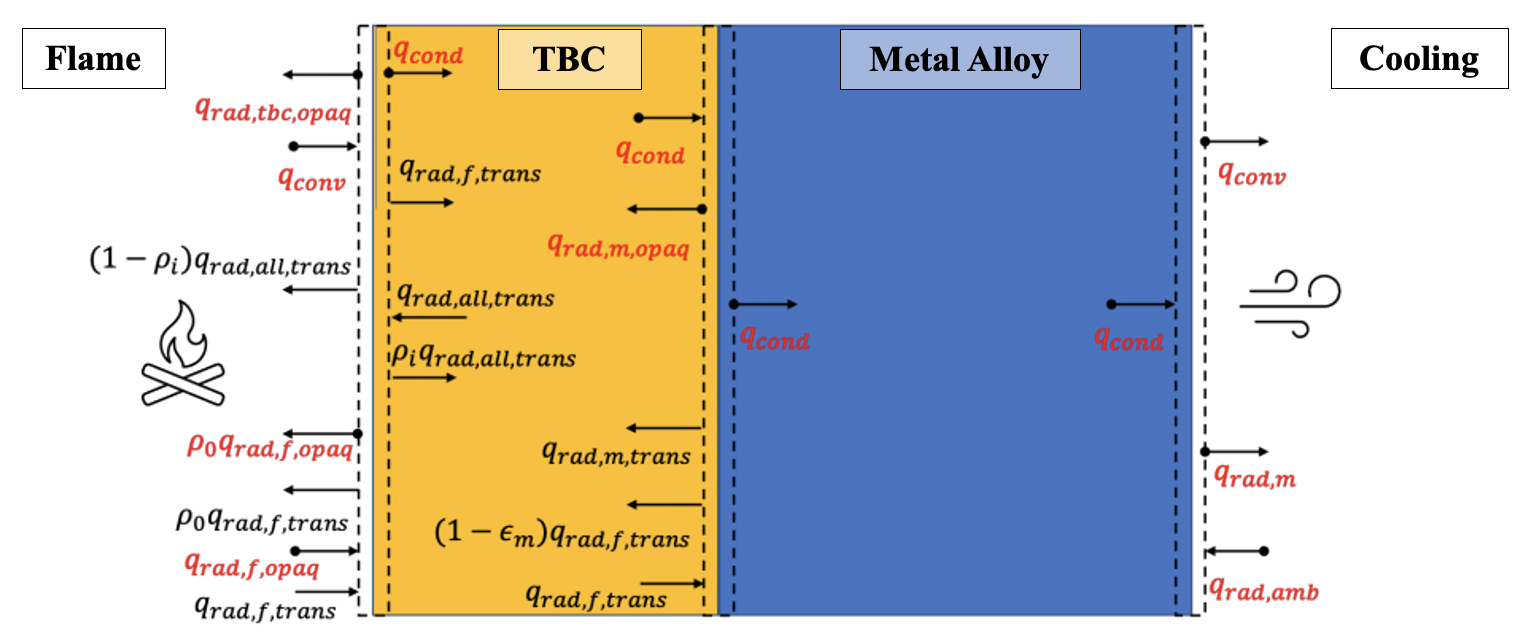
\includegraphics[width=1\linewidth]{figures/ch2/TBC.png}
\caption{The computational domain for the conjugate heat transfer solver from~\cite{Tricard2021ModelingEnvironments.}. Various sources of heat transfer rate are labeled, with the red-fonted heat transfer rates accounted for by the conduction solver and the black-fonted heat transfer rates accounted for by the radiation solver. The yellow domain and blue domains are the TBC and metal, respectively. The x direction follows from the flame to the impingement flow. The y and z directions are vertical and into the page, respectively. }
\label{fig:TBC}
\end{figure}

\subsection{On chemistry}
Combustion processes are highly coupled to the accompanying complex chemical reaction network.
The network of reactions that proceed during the conversion from a large hydrocarbon molecule to the smaller product species produces inherit complexities during the modeling procedure, especially in relation to the existing macroscopic thermodynamic properties used to define these mixtures.
Radiation has been previously shown to influence the temperature of a system. Temperature has a high degree of influence on the rapid chemical processes undergone in the reaction.
This presents an additional, indirect, influence of radiation on the combustion process . One that requires modeling of full modeling of thermal, fluidic, and chemical processes within the combustion simulation for an adequate analysis.

The obvious influence on temperature influences the product species concentrations at the exit of many combustion systems. In particular, the production of pollutant species NO$_x$ (nitrous oxides) and soot can be significantly affected \cite{Viskanta2010RadiativeSystems}.

\citet{Ihme2008ModelingFormulation} demonstrated the influence of radiation on NO$_x$ production by including an additional dimension to the flamelet progress variable approach for chemistry tabulation.
They applied the optically thin assumption (OTA), where only radiative emission is considered, to simulations of the Sandia D. flame, and the Pratt \& Whitney PW6000 combustor without accounting for turbulence-radiation interaction.
For both cases, production of nitric oxide was reduced as a result of the lower temperatures.

\citet{Wu2021LimitationsFires} later highlighted the importance of including radiative absorption in these simulations using a budget analysis of relative contributions of various physics on temperature. 
They used mixture fraction ($Z$), a quantity to quantify the mixing between fuel ($Z=1$) and oxidizer ($Z=0$), to demonstrate the range of contributions of emission and absorption.
It was shown that radiative emission is very high near the stoichiometric mixture fraction, but decreases quickly around the fuel-rich and fuel-lean sides of the flame. Radiative absorption, in contrast, retains its magnitude across the mixture fraction range.
Additionally, to reduce the computational intensity of joint combustion-radiation calculations, they developed a cylindrical flamelet model to pre-tabulate the contribution of radiation to the pool-fire simulation with promising results.
This provides a useful route of future research as spectral absorption coefficient and black body emission can be obtained using mixture fraction and temperature alone \cite{Viskanta2010RadiativeSystems}.

